\subsection{Descripción del problema}
Uno de los principales efectos del reciente boom tecnológico del siglo XXI ha sido la facilidad que tiene propagar información. Mediante redes sociales, grupos de \textit{chats}, páginas web, la simplicidad con la que diferentes artículos, comentarios, imágenes, videos, etc. se difunden es asombrosa. Si bien esto es una ventaja para la globalización y la compartición de conocimiento, es también una herramienta para divulgar información no verídica que busca confundir, desorientar y, ciertamente, modificar las realidades del mundo. Quienes propagan esta información falsa no siempre son conscientes de ello, pues en la gran mayoría de los casos son personas que se fijan en la veracidad de las fuentes u otras características que evidenciarían que la información es falsa.\\

Surge entonces el problema de poder detectar estas noticias falsas, buscando detener la propagación de la desinformación que en algunos casos podría traer consecuencias realmente nefastas, en especial cuando se trata de temas de salud, como posibles curas o remedios caseros para algún tipo de enfermedad. La historia reciente de la humanidad lidiando con la pandemia del Sars-CoV-2 o COVID19 trajo, entre muchos, un caso polémico en que el Expresidente de Estados Unidos sugería la utilización de desinfectante inyectado para tratar el virus, lo cual desencadenó una serie de eventos desafortunados de personas intoxicadas por seguir la recomendación. Por otra parte, existe la reciente notificación por parte de OpenAI acerca de los resultados de generación de texto de la red GPT3 cuyos pesos e hiperparámetros no hicieron públicos justamente por la posibilidad de utilizarla para generar información falsa y posteriormente difundirla.\\

Actualmente, hay algunos \textit{datasets} diseñados para entrenar modelos para cumplir la tarea de detección de noticias falsas. Sin embargo, la gran mayoría están basados en publicaciones de redes sociales, las cuales si bien son uno de los principales medios de difusión, excluyen por completo la importante consideración a tener en cuenta respecto a la generación de noticias falsas mediante redes profundas como GPT o similares. Es por esta razón que para el desarrollo del presente proyecto se decide utilizar únicamente noticias generadas por modelos de inteligencia artificial, etiquetadas como falsas, y noticias reales recopiladas de fuentes confiables, etiquetadas como verdaderas.\\

A continuación, se describen a detalle diferentes etapas del proceso de solución al problema de detección de noticias falsas.

\subsection{Revisión del estado del arte}
Actualmente, de acuerdo con \cite{PapersWithCodeBenchmark} existen cuatro tareas famosas en detección de noticias falsas:
\begin{enumerate}
    \item \textit{FNC-1 Stance Detection:} Fue el más utilizado hasta hace tres años. Consiste en detectar la postura de un documento con respecto a una afirmación del usuario.
    \item \textit{Grover Mega} \cite{grover}\textit{:} Es un proyecto de la universidad de Washington en que se trabaja con todos los temas relacionados con Fake News, desde generación hasta detección.
    \item \textit{Fake news and hostility detection:} Tarea propuesta recientemente, pero con poca participación debido a que el \textit{dataset} esta en árabe.
    \item \textit{Fake News Detection on COVID19 related dataset:} Detección de noticias falsas relacionas con COVID19. El \textit{dataset} consiste en una recopilación de \textit{tweets} de cuentas oficiales de noticias y de otras con fama de divulgar noticias falsas.
\end{enumerate}

Teniendo en cuenta los objetivos del proyecto se le da mayor importancia a la última tarea y al estado del arte relacionado con la misma, el cual se divide en dos grandes grupos dependiendo del acercamiento que da cada artículo al problema.

\subsubsection{Técnicas de clasificación:}
Los artículos de este grupo se enfocan en aplicar diferentes algoritmos de clasificación, utilizando como base técnicas tradicionales de extracción de características \cite{List2, List1, Constraint, List3, List4, FightingInfodemic}. En su gran mayoría utilizan \textit{embeddings} como Doc2Vec como extractor de características, sin descartar en algunos casos la utilización de TF-IDF. En cuanto a qué técnicas de \textit{Machine Learning} se utilizan, se rescatan SVM, Naïve Bayes, Logistic Regression, redes neuronales, entre otros.\\

En cada uno de los artículos previamente referenciados puede verse una comparación de los resultados obtenidos con los diferentes modelos y en algunos casos con diferentes técnicas de extracción de características. Los mejores resultados tomando como punto de comparación la métrica F1-score los obtiene una red neuronal implementada en \textit{TensforFlow} con un puntaje de 0,94. El modelo que mejor resultado alcanza sin tener en cuenta redes neuronales es un SMV con 0,9381. 

\subsubsection{Técnicas de extracción de características:}
El segundo grupo de artículos corresponde a investigaciones mucho más profundas en un único método completo, desde preprocesamiento del \textit{dataset} pasando por el proceso de extracción de características, donde más énfasis y, finalmente, diseño, implementación y evaluación del modelo de clasificación.\\ A continuación, se detalla el proceso seguido por algunos documentos que presentan excelentes resultados:

\begin{itemize}
    \item \cite{XLNetCovid} propone la utilización de un clasificador sencillo compuesto únicamente por dos capas densas (\textit{fully connected}). La principal contribución es la propuesta de utilizar LDA (\textit{Latent Dirichlet Allocation)} y XL-Net (una red del estado del arte) para extraer características de cada uno de los textos. Los resultados de este artículo alcanzan 0.967 F1-score.
        
    \item \cite{Heuristic} utiliza un ensamblaje de redes del estado del arte, especialmente variaciones de BERT(CT-BERT, RoBERT, BERT, etc.) para hacer la clasificación de cada texto. Finalmente, realiza un proceso de votación con ponderación de probabilidades o con conteo de respuestas positivas o negativas de las diferentes redes. El resultado de F1-score es 0.9813.
        
    \item \cite{TranformerBasedFineTuning} propone un acercamiento en el que se tengan en cuenta frases profesionales específicas del dominio que se está trabajando, posteriormente utilizar un entrenamiento con una función \textit{softmax} con temperatura incrementada. Después de ello, se utiliza entrenamiento adversarial en que se agrega ruido bajo una función específica para intentar engañar a la red, y con ello darle mayor robustez. Finalmente, utilizan un ensamblaje de diferentes modelos de BERT para extraer las características de cada texto. Estas características son la entrada de un clasificador pequeño y sencillo cuyo resultado es de 0.9901 F1-score.
\end{itemize}

\subsection{Generación de datos sintéticos}
Como se mencionó en la descripción del problema, en el caso específico del proyecto se desea enfocar el trabajo a la detección de FakeNews específicamente cuando se trata de noticias falsas generadas por redes profundas del estado del arte, GPT2 específicamente. A continuación, se presenta el paso a paso del proceso de generación de noticias falsas.\\

En primer lugar, se decidió hacer uso de la librería Transformers especialmente por su facilidad para crear un \textit{pipeline} que permita generar texto. Para ello únicamente se debe especificar el modelo que se desea utilizar el cual viene preentrenado para la tarea de generación de texto. En este caso se seleccionaron modelos específicamente para cada idioma según la oferta en la página web de la librería. Posteriormente, se debe proveer una oración inicial sobre la que se basará el modelo para generar texto. Este contexto se creo tomando como base el título y las primeras oraciones de algunas de las noticias reales recopiladas en la primera etapa del proyecto. \\

Se preparó entonces un script que genera una noticia falsa para cada uno de los archivos indicados, y con un modelo seleccionado dependiendo del idioma a trabajar. A pesar de que la generación se realizó utilizando GPU, el proceso fue bastante demorado (+/- 5 segundos por iteración), razón por la cual se generaron un número menor de noticias falsas.

\subsection{Extracción de características}
El proceso de extracción de características de cada documentos se realizó en primera instancia mediante técnicas tradicionales: TFIDF y \textit{Bag of words} con el fin de comparar con los resultados obtenidos en los artículos del primer grupo del estado del arte previamente descrito. Para ello se utilizó la librería \textit{Scikit-learn} y su función de \textit{text feature-extraction}. Se indicó que se deben retirar las \textit{stopwords} de cada uno de los idiomas intentados y retirar también las palabras que aparecen menos de 30 veces en el corpus. El procedimiento es bastante veloz para la extracción de características, a pesar de no ser muy eficiente en el manejo de memoria, como se ha mencionado en tareas previas. Tiene la notable ventaja de que no hay necesidad de recortar los documentos, pues la única consecuencia de un documento largo es que la normal de los vectores será un poco mayor,  pero no representa un problema, mientras que la tokenización con modelos preentrenados sí.\\

Como estrategia adicional de extracción de características se decidió hacer uso de un modelo preentrando disponible en la librería \textit{Transformers}. De manera similar a como se implementó en el primer punto del proyecto, se define el modelo y se extrae los \textit{embeddings} de la capa correspondiente a los \textit{embeddings} del documento. No obstante, esta estrategia presenta el grave problema de que es necesario recortar los documentos a un número específico de tokens para que la red reciba las entradas, lo que ocasiona fuerte pérdida de información. No obstante, se realizaron ensayos con ambos métodos de extracción de características y se evaluaron sus resultados. A continuación, se detallan los métodos de clasificación utilizados.

\subsection{Modelos de clasificación}
Siguiendo con las propuestas detalladas en el estado del arte, se decide probar el desempeño de diferentes clasificadores como \textit{Logistic Regression}, \textit{Naïve Bayes}, \textit{Multilayer Perceptron} y \textit{Support Vector Machines}. Cada uno de ellos, con las diferentes propuestas de extracción de características previamente mencionadas. De cada uno de los doce experimentos se obtienen medidas de \textit{accuracy}, \textit{precision}, \textit{recall} y \textit{f1-score}, siendo este último el más importante, con el fin de poder comparar los resultados con los artículos presentados en la revisión bibliográfica del estado del arte.

\subsection{Resultados}
Como se describió previamente, evalúan los resultados obtenidos por diferentes modelos con diferentes métodos de extracción de características. En cada caso se evalúan \textit{accuracy}, \textit{precision}, \textit{recall} y \textit{f1-score}. Se muestran a continuación los resultados consolidados de los modelos evaluados y por último se concluirá sobre el mejor modelo (método de extracción de características y algoritmo de ML) para atacar este problema específico.

\input{results/FakeNewsDetection/results-df.txt}

\subsubsection{Comparación por método de extracción de características}
\begin{figure}
    \centering
    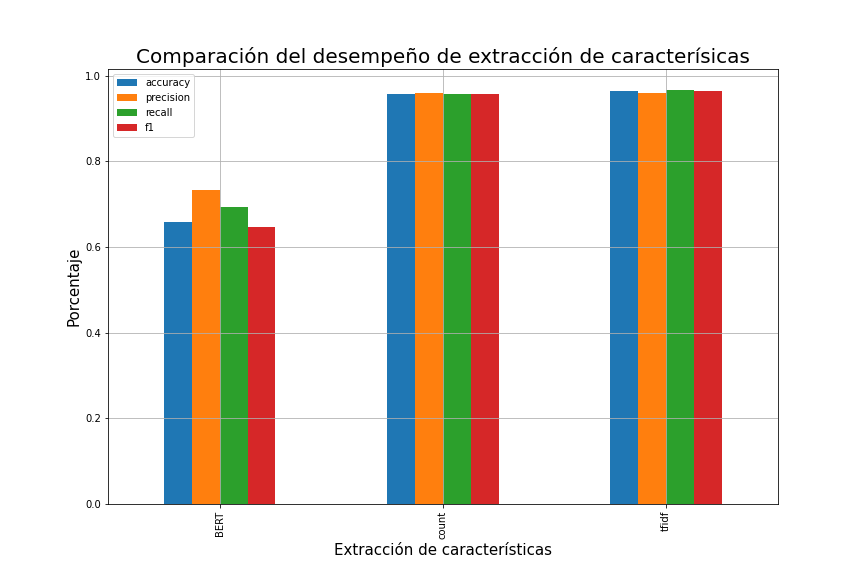
\includegraphics[width=\textwidth]{results/FakeNewsDetection/feature_extraction_comparison.png}
    \caption{Comparación de métodos de extracción de características}
    \label{fig:fake_news_feature_extraction}
\end{figure}

Como se muestra en la figura \ref{fig:fake_news_feature_extraction}, es evidente que el método de tokenización usando BERT no da resultados tan buenos como \textit{Bag of words} o \textit{TF-IDF}. Esta diferencia se debe a que el modelo BERT no fue ajustado ni afinado para el \textit{dataset} específico con el que se está trabajando actualmente, mientras que los otros dos fueron creados directamente teniendo en cuenta los documentos disponibles para la tarea. Se esperaría que los resultados al tener un modelo con la capacidad de BERT afinado específicamente para esta tarea mejoren notablemente, incluso superando los resultados de los otros dos métodos de extracción de características.

\subsubsection{Comparación por modelo de ML}
\begin{figure}
    \centering
    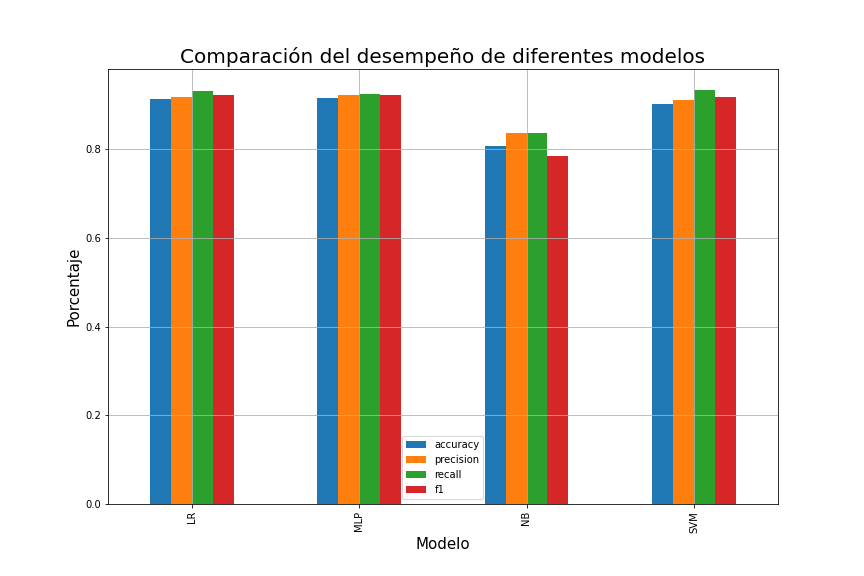
\includegraphics[width=\textwidth]{results/FakeNewsDetection/model_comparison.png}
    \caption{Comparación de modelos de ML}
    \label{fig:fake_news_models}
\end{figure}

La diferencia entre el desempeño de los modelos utilizados (\textit{véase fig. \ref{fig:fake_news_models}}) no es tan evidente como el caso previo de extractores de características. Regresión logística, red neuronal y máquina de soporte vectorial presentan resultados muy similares y buenos, mientras que \textit{Naïve Bayes} está ligeramente rezagado en resultados. No obstante, es necesario resaltar la velocidad de entrenamiento de NB. Esta diferencia puede atribuirse a que el único modelo generativo es NB, siendo todos los demás discriminativos. Esto da una idea de que el problema de detección de \textit{Fake News} es más bien discriminativo.

\subsubsection{Comparación por idioma}
\begin{figure}
    \centering
    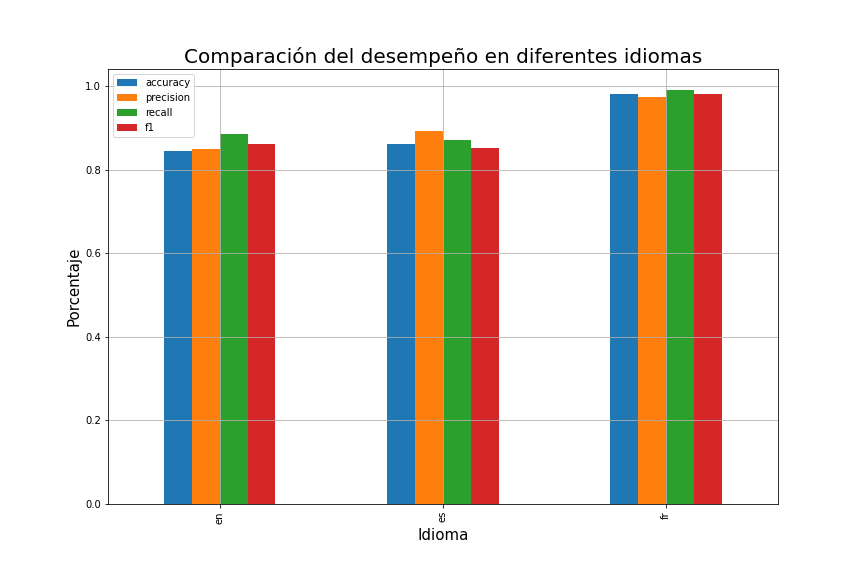
\includegraphics[width=\textwidth]{results/FakeNewsDetection/language_comparison.png}
    \caption{Comparación de idiomas}
    \label{fig:fake_news_languages}
\end{figure}

En cuanto a los idiomas, el resultado de la comparación indica que francés tiene ligeramente mejores resultados para la clasificación de noticias falsas y español e inglés tiene resultados muy similares (\textit{véase fit. \ref{fig:fake_news_languages}}). En primera instancia, se esperaba que el resultado de inglés fuera el mejor debido a que es un idioma de cierta forma más sencillo, en especial en cuanto a conjugación de verbos. No obstante, los resultados podrían explicarse con base en que así como francés es un idioma más difícil de representar, debe ser más difícil de tokenizar y por tanto debe presentar más dificultades para su generación, facilitando la distinción de noticias generadas sintéticamente y noticias reales escritas por personas que dominan la lengua.

\subsection{Conclusiones}
Los resultados obtenidos son buenos. En algunos casos se supero con creces un f1-score de 0.95, sobrepasando resultados de los artículos mencionados en el primer grupo del estado del arte. Incluso hay dos modelos que tienen un desempeño perfecto en todas las métricas. No obstante, la tokenización con BERT no tuvo un resultado tan bueno como se esperaba y como los artículos del segundo grupo presentaban. La razón a la que se le atribuye esta diferencia es a que no se realizó una afinación del modelo para trabajar específicamente con este \textit{dataset}, lo cual se espera que mejoraría su funcionamiento.\\

Con base en los resultados obtenidos por la gran mayoría de modelos, en especial al tokenizar con técnicas tradicionales, podría decirse que la tarea de identificar \textit{Fake News} generadas por redes neuronales no es tan difícil. Ahora bien, a medida que las técnicas de generación de texto van mejorando, puede que se convierta en una tarea más complicada.\\

El trabajo de detección de \textit{Fake News} es una tarea reciente y tiene mucho trabajo futuro. Para el caso específico de este proyecto se rescata la afinación del modelo de extracción de características al igual que la posible utilización de otros \textit{embeddings} como Word2Vec o Doc2Vec, entrenados específicamente sobre el \textit{dataset} trabajado. Así mismo, podría estudiarse la posibilidad de entrenar una red de generación de texto específicamente en la tarea de generar noticias falsas, quizás complicando su distinción. Adicionalmente, podrían juntarse datos de diferentes fuentes como \textit{Twitter}, noticias falsas escritas por personas y noticias falsas escritas por redes neuronales profundas, con el objetivo de poder proporcionar un modelo capaz de realizar una distinción total, sin importar su origen.
